\section{Cloud Computing}
Seit der Entstehung des Begriffs \glqq Cloud Computing\grqq{} haben IT Firmen oder öffentliche Institute unterschiedliche Definitionen für den Begriff formuliert. Der Grundgedanke von Cloud Computing ist es jedoch Ressourcen oder Dienste über ein Netzwerk bereitzustellen oder zu nutzen. Cloud Computing kann folgendermaßen definiert werden: Cloud Computing ist die Bereitstellung von Rechenressourcen über das Internet. Die Cloud Dienste ermöglichen sowohl Privatpersonen als auch Unternehmen Software oder Hardware zu nutzen, welche von einer außenstehenden Partei an einem anderen Standort zur Verfügung steht\cite{canada}. Cloud Computing ist per Definition eine spezifische Methode um skalierbare IT-bezogener Funktionen bei Bedarf über das Internet für mehrere Benutzer gleichzeitig nutzbar zu machen\cite{gartner}.
Wie man sieht, gibt es keine einheitliche Definition für den Begriff \glqq Cloud Computing\grqq, jedoch hat sich die Definiton des amerikanischen National Institute of Standards and Technology (NIST) als weitläufig anerkannt herausgestellt. Das NIST bezeichnet Cloud Computing demnach als ein Modell, das einen einfachen und bedarfsgesteuerten Zugriff über ein Netzwerk zu einem geteilten Pool aus konfigurierbaren Rechenressourcen (bspw. Netzwerke, Server, Speicherplatz, Anwendungen und Dienste) ermöglicht. Diese Ressourcen sollen mit minimalen Verwaltungsaufwand oder durch den Dienst Provider bereitgestellt werden können. Cloud Computing setzt sich aus 5 Eigenschaften, 3 Dienstmodellen und 4 Einsatzmodellen zusammen\cite{nist_definition}.

\subsection{Eigenschaften} 

\textbf{Selbstbedienung auf Nachfrage} \hfill 
Ein Verbraucher kann sich selbst Rechenressourcen bereitstellen ohne mit einem Mitarbeiter des Anbieters kommunizieren zu müssen\cite{nist_definition}.

\textbf{Breiter Netzwerkzugang} \hfill
Ressourcen sind über das Netzwerk verfügbar und können über Standardmechanismen von heterogenen Clients genutzt werden\cite{nist_definition}.

\textbf{Ressourcen Vereinigung} \hfill
Die Rechenressourcen des Anbieters sind gebündelt, um mehrere Verbraucher zu bedienen und ihnen dynamisch physikalische oder virtuelle Ressourcen auf Nachfrage zuzuweisen. Dafür wird ein Multi-Tenant-Modell benutzt. Diese Ressourcen sind beispielsweise Speicherplatz, Rechenleistung oder Netzwerkbandbreite. Der Verbraucher hat in der Regel keine Kenntnis darüber, wo sich die bereitgestellten Ressourcen befinden. Dennoch kann es sein, dass er den Standort eingrenzen kann bspw. auf ein Land oder ein Rechenzentrum\cite{nist_definition}.

\textbf{Schnelle Elastizität} \hfill
Die Ressourcen können dehnbar freigegeben und bereitgestellt werden, teilweise automatisch, um entsprechend der Nachfrage skalieren zu können\cite{nist_definition}.

\textbf{Messbarer Service} \hfill
Die Cloud-Systeme steuern automatisch die Ressourcennutzung durch Verwendung einer Messkapazität. Je nach Dienst bietet sich hierfür unterschiedliche Werte an, dies kann beispielsweise der Speicher oder aktive Benutzerkonten sein. Die Ressourcennutzung kann überwacht, kontrolliert und protokolliert werden, somit kann sowohl für den Verbraucher als auch für den Anbieter Transparenz für die Nutzung des benutzten Dienstes geschaffen werden\cite{nist_definition}.


\subsection{Dienst Modelle}
\textbf{Software as a Service (SaaS)} \hfill
Der Kunde hat hier die Möglichkeit, die bereitgestellten laufenden Anwendungen der Infrastruktur des Anbieters zu nutzen. Diese Anwendungen sind durch Client-Anwendungen über eine Schnittstelle erreichbar. Der Verbaucher hat keine Kontrolle über die darunterliegende Infrastruktur, sprich Netzwerk, Server, Betriebssysteme, Speicherplatz oder individuelle Anwendungseinstellungen mit Ausnahme eingeschränkter anwenderspezifischer Einstellungen\cite{nist_definition}.

\textbf{Platform as a Service (PaaS)} \hfill
Der Kunde hat hier die Möglichkeit, eigens entwicklte oder erworbene Anwendungen auf der Infrastruktur des Anbieters bereit zu stellen. Der Verbaucher hat keine Kontrolle über die darunterliegende Infrastruktur, sprich Netzwerk, Server, Betriebssysteme, Speicherplatz. Aber er hat die Kontrolle über individuelle Anwendungseinstellungen sowie anwenderspezifische Einstellungen\cite{nist_definition}.

\textbf{Infrastructure as a Service (IaaS)} \hfill
Der Kunde bekommt vom Anbieter die Infrastruktur bereitgestellt um Operationen durchzuführen, dazu gehören Speicher, Hardware, sowie Netzwerk. Die Infrastruktur kann der Verbaucher benutzen um willkürliche Software darauf zu verwenden, einschließlich Betriebssysteme und Anwendungen. Der Verbaucher hat keine Kontrolle über die darunterliegende Infrastruktur, sprich Netzwerk und Hardware, aber er hat die volle Kontrolle über das Betriebssystem, Anwendungen, Speicher und möglicherweise eingeschränkten Zugriff auf die Netzwerkkomponenten beispielsweise Firewall-einstellungen\cite{nist_definition}.

\begin{figure}[H]
	\centering
	\includegraphics[width=0.45\textwidth]{Images/Iaas}
	\caption{Services}
	\label{Services}
\end{figure}
\begin{figure}[H]
	\centering
	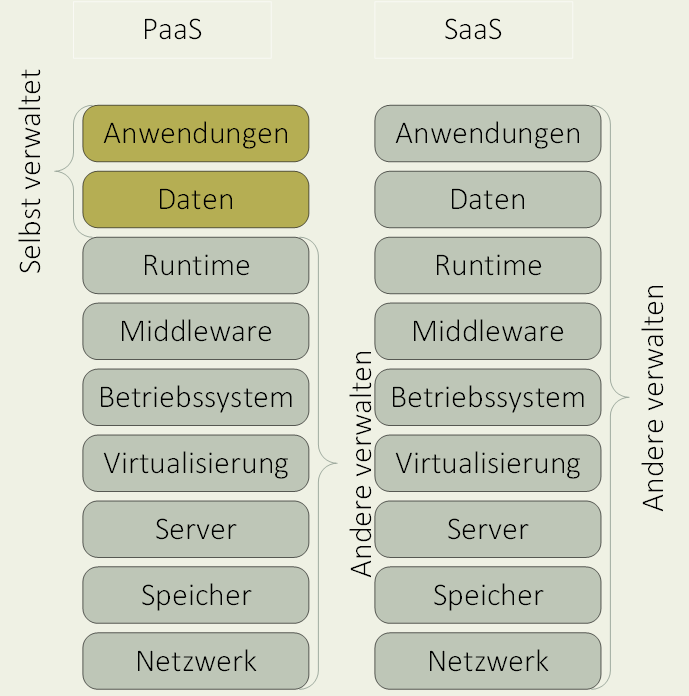
\includegraphics[width=0.45\textwidth]{Images/SaaS}
	\caption{Services}
	\label{Services}
\end{figure}

\subsection{Kategorien}
\subsubsection{Private Cloud}
Diese Art von Cloud-Infrastruktur wird aussschließlich für eine einzige Organisation und ihren Mitarbeitern bereitgestellt. Die Infrastruktur kann besitzt, verwaltet und betrieben werden von der Organisation selbst, einer dritten Partei oder eine Kombination der beiden. Dabei kann die Infrastruktur innerhalb oder außerhalb der Räumlichkeiten der Organisation liegen\cite{nist_definition}.

\subsubsection{Community Cloud}
Diese Art von Cloud-Infrastruktur wird aussschließlich für eine spezielle Gemeinschaft an Verbrauchern mit einem gemeinsamen Interesse (bspw. Sicherheitsanforderungen oder Richtlinien) bereitgestellt. Die Infrastruktur kann besitzt, verwaltet und betrieben werden von einer oder mehreren Organisationen der Gemeinschaft selbst, einer dritten Partei oder eine Kombination der beiden. Dabei kann die Infrastruktur innerhalb oder außerhalb der Räumlichkeiten der Organisationen liegen\cite{nist_definition}.

\subsubsection{Public Cloud}
Diese Art von Cloud-Infrastruktur wird für die Öffentlichkeit bereitgestellt. Die Infrastruktur kann besitzt, verwaltet und betrieben werden von einem Unternehmen, staatlichen Einrichtung oder eine Kombination der beiden. Die Infrastruktur befindet sich in den Räumlichkeiten des Cloud-Providers\cite{nist_definition}. Ein Teil der Service-Infrastruktur wird in der private Cloud bewältigt und ein anderer Teil in der Public Cloud. Das bietet eine bessere Kontrolle über die Daten und dennoch eine Möglichkeit Ressourcen nach Bedarf zu nutzen\cite{study_cc_cdb}.

\subsubsection{Hybrid Cloud}
Diese Art von Cloud-Infrastruktur ist ein Verbund aus zwei oder mehreren Cloud-Infrastrukturen(private,community oder public), welche weiterhin einzeln bestehen, aber mithilfe von standardisierten oder propietären Technologien die Portabilität von Daten und Anwendungen ermöglichen\cite{nist_definition}.


